\section{Velocity Transformations}
%By Matt Trawick.

\instructornote{%
By Matt Trawick, 2021.  Time: 30 minutes?

I wrote this for my FYS class in 2021.  I intended it as an easy lab, and probably not really necessary for Modern.
But it turns out that students seemed to get a lot out of it.  Maybe I'll use it in Modern too.
}

\makelabheader %(Space for student name, etc., defined in master.tex)

\bigskip

\textbf{Activity 1: Faster Than Light?}

\begin{enumerate}[labparts]
\item Suppose Bob is standing on the ground and aims a laser in the positive $x$ direction, just as Anna zooms by on a train going in the negative $x$ direction at velocity $v=-0.6c$.  What will Anna measure as the speed of the laser beam?
\answerspace{0.5in}

Tired of always measuring the same speed, Anna and Bob try a new experiment.  Bob stands on the ground again, but this time he throws a baseball with a velocity $u=+0.8c$ in the positive $x$ direction.  As before, Anna rides a train at velocity $v=-0.6c$ in the opposite direction, as shown below.

\begin{center}
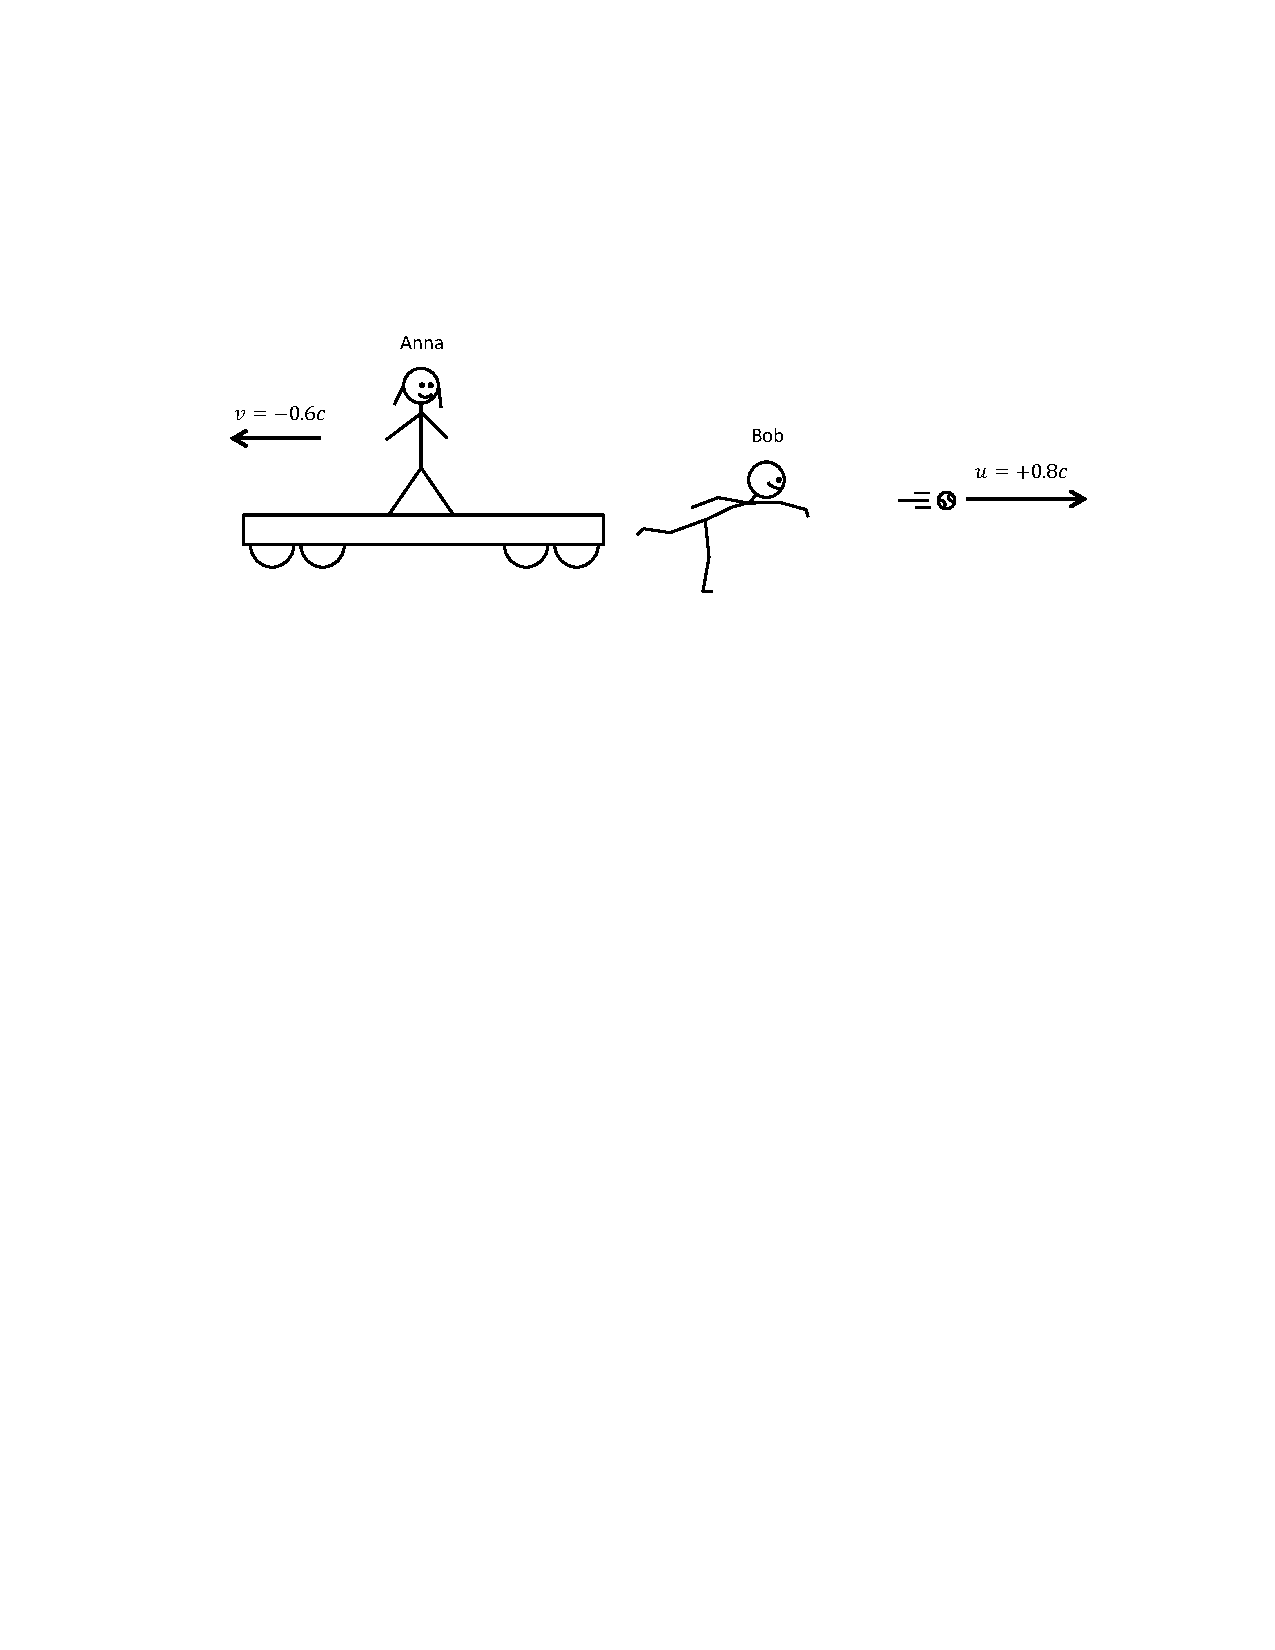
\includegraphics{velocity_transformations/baseball1.pdf}
\end{center}

\item According to the \textit{Galilean transformations}, what would Anna see as the velocity of the baseball?
\answerspace{0.5in}

\item Does it make sense that Anna would see the baseball traveling at \textit{faster} than the laser beam traveled?
\answerspace{0.5in}
\end{enumerate}

\textbf{Activity 2: Some Computer Simulations}

Open the file \filename{velocity\_transformations.nb}.  You may need to hit Ctrl-A to select all, and then Shift-Enter to run the code.  You should see a graph showing many colored worldlines of object traveling at different velocities.  The velocities shown are evenly spaced at intervals of $\pm0.1c$, from $-0.9c$ to $+0.9c$.

\begin{enumerate}[labparts]
\item One of the red lines in the graph would be the worldline for the baseball at $u=+0.8c$ in Bob's reference frame.  Use the slider in the Galilean transformation simulator to show what the ball's velocity would be in Anna's reference frame using the (incorrect) Galilean transformations.  Is your result consistent with your answer in part (b) above?
\answerspace{0.5in}

\item Now view the same situation using the Lorentz transformation simulation.  Based on the simulation, give an \textit{approximate} value below for the velocity of the baseball in Anna's reference frame.
\answerspace{0.5in}

\item Use the Lorentz velocity transformation,
$$u'=\cfrac{u-v}{1-\cfrac{uv}{c^2}}\,,$$
to calculate the exact value of the baseball's velocity in Anna's reference frame.  
\answerspace{1.5in}

\item Does your answer above seem consistent with the value you estimated from the computer simulation?
\answerspace{0.5in}
\end{enumerate}

\textbf{Activity 3: A New Direction}

Now Bob and Anna try a new variation on the experiment.  Bob throws the baseball in the positive $x$ direction with velocity $u=+0.8c$ as before, but this time Anna rides the train in the \textit{same} direction as the ball, with velocity $v=+0.6c$.

\begin{enumerate}[labparts]
\item What would Anna measure for the velocity of the baseball, using the (incorrect) Galilean velocity transformation?
\answerspace{0.5in}

\item Without either doing a calculation or looking at the computer simulation, make a prediction: Using the correct Lorentz velocity transformation, would the velocity of the baseball in Anna's reference frame be \textit{less than} $0.2c$, \textit{equal to} $0.2c$, or \textit{greater than} $0.2c$?  (This is hard.  Think for a bit and make a guess.  No biggie.)
\answerspace{0.5in}

\item Now test your prediction using the Lorentz transformation on the computer simulation.  Was your prediction correct?  \textit{Approximately} what would Anna measure as the baseball's velocity in her reference frame?
\answerspace{0.5in}

\item Calculate the exact value of the velocity $u'$ of the baseball in Anna's reference frame, using the Lorentz velocity transformation equation above.
\answerspace{1.5in}

\item Does your answer above seem consistent with the value you estimated from the computer simulation?
\answerspace{0.5in}
\end{enumerate}

\textbf{Activity 4: Maybe, possibly, faster than light?}

Anna and Bob are determined to measure a speed greater than $c$, \textit{just once}!  So they come up with a plan: This time Bob will ride on the train in the positive $x$ direction at velocity $+0.6c$.  While riding on the train, he will throw the ball at $+0.8c$ relative to himself.  Anna will stand by the side of the tracks and measure the velocity of the ball.

\begin{center}
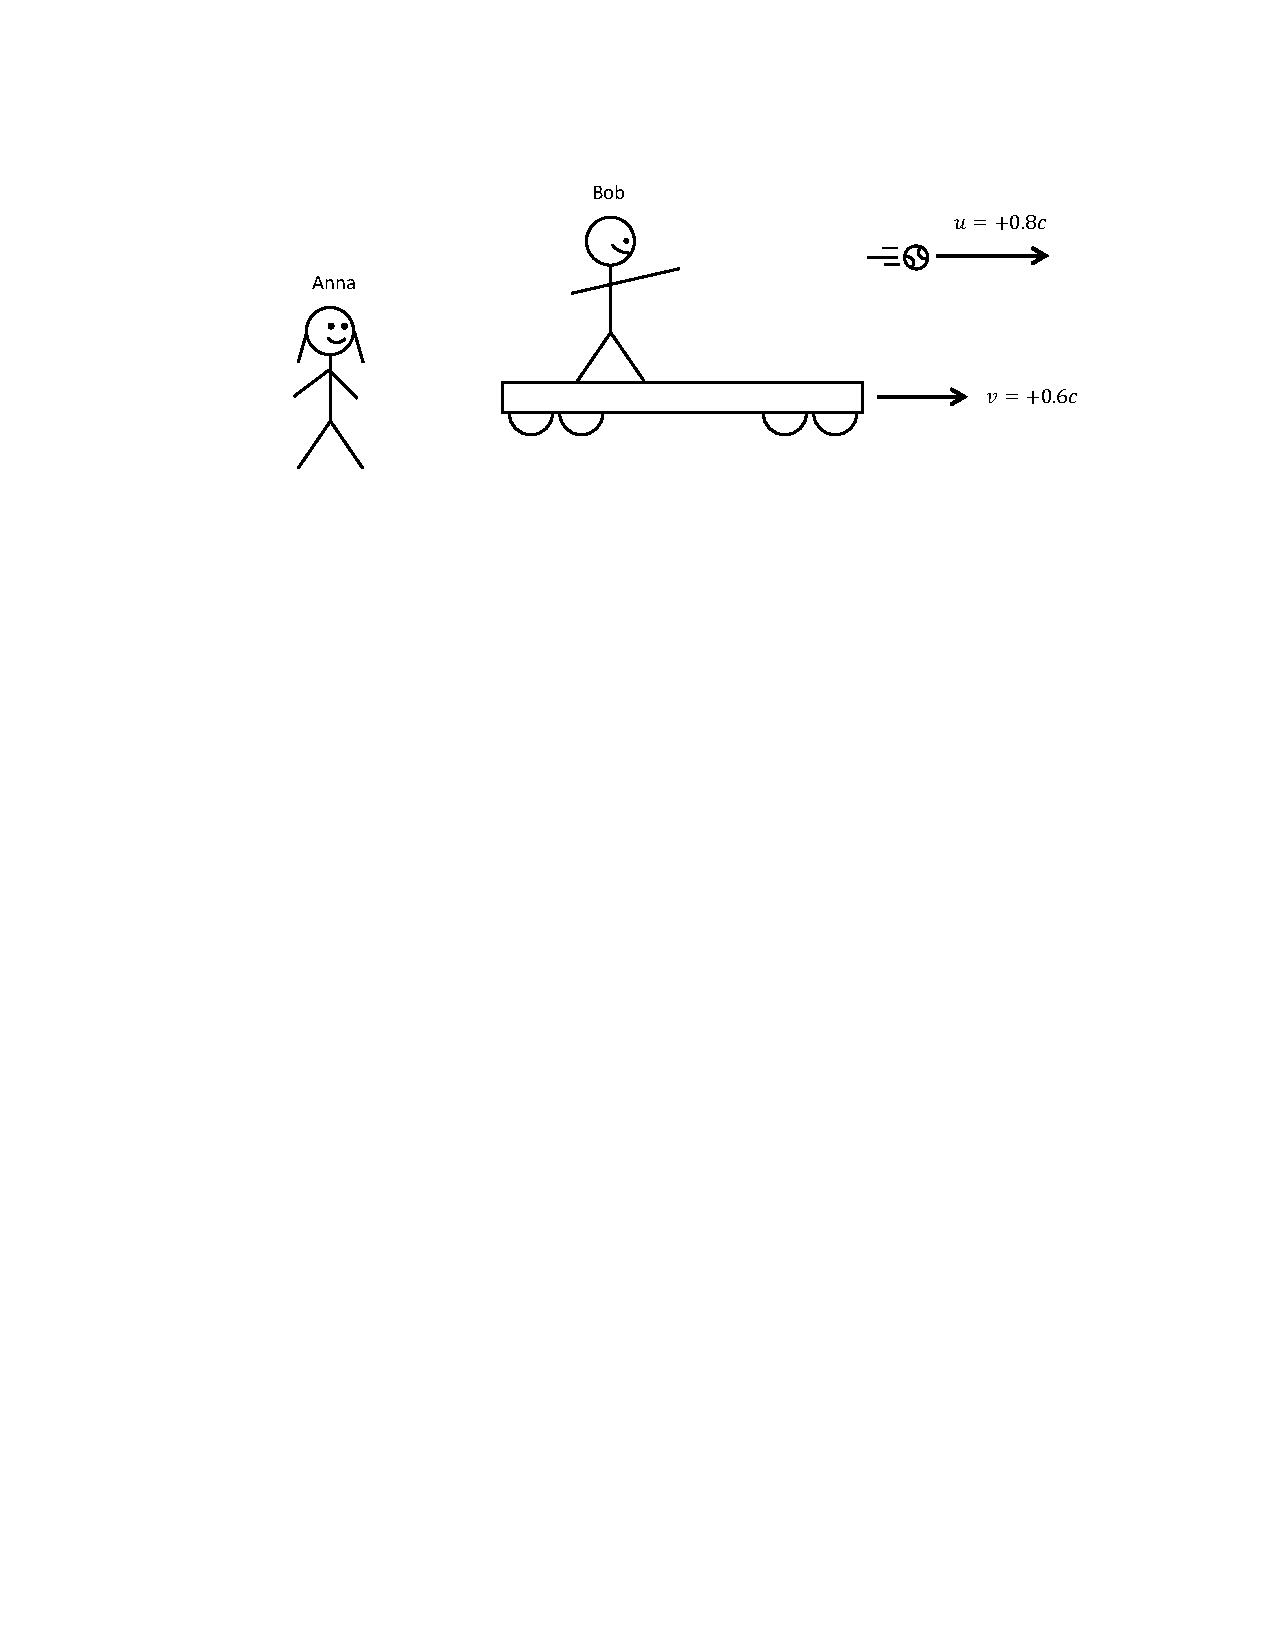
\includegraphics{velocity_transformations/baseball2.pdf}
\end{center}

\begin{enumerate}[labparts]
\item Make a prediction: Do you think Anna will measure a velocity greater than $c$ for the baseball?
\answerspace{0.5in}

\item The picture above is actually misleading (that is, it's wrong!), because the labels of the velocity vectors are in two different reference frames.  Bob sees the ball at $u=+0.8c$, but in Bob's reference frame the train car is not moving.  Meanwhile, Anna sees the train moving forward at $+0.6c$, but she surely doesn't see the ball at $0.8c$.  In the space below, make two separate drawings showing Anna, Bob, the train, and the ball: one in Bob's reference frame, and one in Anna's reference frame.  Include velocity vectors and labels showing the correct speeds of Anna, Bob, and the ball as seen in each reference frame.  

\hspace{\fill}Anna's frame\hspace{\fill}\rule{1pt}{3in}\hspace{\fill}Bob's frame\hspace{\fill}

\item Compare your drawing of Bob's reference frame to the very first diagram on the first page of this lab.  Other than who happens to be on the train, is there any difference between the two drawings?
\answerspace{0.5in}

\item What velocity does Anna measure for the baseball?
\answerspace{0.5in}

\end{enumerate}


